\subsection{x86}

\subsubsection{\NonOptimizing MSVC}

\RU{Итак, компилируем:}\EN{Let's compile:}

\lstinputlisting{patterns/10_strings/1_strlen/10_1_msvc.asm.\LANG}

\index{x86!\Instructions!MOVSX}
\index{x86!\Instructions!TEST}
\RU{Здесь две новых инструкции: \MOVSX и \TEST.}
\EN{We get two new instructions here: \MOVSX and \TEST.}

\label{MOVSX}
\RU{О первой. \MOVSX предназначена для того, чтобы взять байт из какого-либо места в памяти и положить его, 
в нашем случае, в регистр \EDX. 
Но регистр \EDX~--- 32-битный. \MOVSX означает \IT{MOV with Sign-Extend}. 
Оставшиеся биты с 8-го по 31-й \MOVSX сделает единицей, если исходный байт в памяти имеет знак \IT{минус}, 
или заполнит нулями, если знак \IT{плюс}.}
\EN{The first one---\MOVSX---takes a byte from an address in memory and stores the value in a 32-bit register. 
\MOVSX stands for \IT{MOV with Sign-Extend}. 
\MOVSX sets the rest of the bits, from the 8th to the 31th, 
to 1 if the source byte is \IT{negative} or to 0 if is \IT{positive}.}

\RU{И вот зачем всё это.}\EN{And here is why.}

\RU{По умолчанию в MSVC и GCC тип \Tchar~--- знаковый. Если у нас есть две переменные, одна \Tchar, а другая \Tint 
(\Tint тоже знаковый), и если в первой переменной лежит -2 (что кодируется как \TT{0xFE}) и мы просто 
переложим это в \Tint, 
то там будет \TT{0x000000FE}, а это, с точки зрения \Tint, даже знакового, будет 254, но никак не -2. 
-2 в переменной \Tint кодируется как \TT{0xFFFFFFFE}. Для того чтобы значение \TT{0xFE} из переменной типа 
\Tchar переложить 
в знаковый \Tint с сохранением всего, нужно узнать его знак и затем заполнить остальные биты. 
Это делает \MOVSX.}
\EN{By default, the \Tchar type is signed in MSVC and GCC. If we have two values of which one is \Tchar 
and the other is \Tint, (\Tint is signed too), and if the first value contain -2 (coded as \TT{0xFE}) 
and we just copy this byte into the \Tint container, it makes \TT{0x000000FE}, and this 
from the point of signed \Tint view is 254, but not -2. In signed int, -2 is coded as \TT{0xFFFFFFFE}. 
So if we need to transfer \TT{0xFE} from a variable of \Tchar type to \Tint, 
we need to identify its sign and extend it. That is what \MOVSX does.}

\RU{См. также об этом раздел}
\EN{You can also read about it in} \q{\IT{\SignedNumbersSectionName}}\EN{ section}~(\myref{sec:signednumbers}).

\RU{Хотя конкретно здесь компилятору вряд ли была особая надобность хранить значение \Tchar в регистре \EDX, 
а не его восьмибитной части, скажем \DL. Но получилось, как получилось. Должно быть 
\gls{register allocator} компилятора сработал именно так.}
\EN{I'm not sure if the compiler needs to store a \Tchar variable in \EDX, it could just take a 8-bit register part 
(for example \DL). Apparently, the compiler's \gls{register allocator} works like that.}

\index{ARM!\Instructions!TEST}
\RU{Позже выполняется \TT{TEST EDX, EDX}. 
Об инструкции \TEST читайте в разделе о битовых полях~(\myref{sec:bitfields}).
Конкретно здесь эта инструкция просто проверяет состояние регистра \EDX на 0.}
\EN{Then we see \TT{TEST EDX, EDX}. 
You can read more about the \TEST instruction in the section about bit fields~(\myref{sec:bitfields}).
Here this instruction just checks if the value in \EDX equals to 0.}

\ifdefined\IncludeGCC
\subsubsection{\NonOptimizing GCC}

\RU{Попробуем}\EN{Let's try} GCC 4.4.1:

\lstinputlisting{patterns/10_strings/1_strlen/10_3_gcc.asm}

\label{movzx}
\index{x86!\Instructions!MOVZX}
\RU{Результат очень похож на MSVC, только здесь используется \MOVZX, а не \MOVSX. 
\MOVZX означает \IT{MOV with Zero-Extend}. Эта инструкция перекладывает какое-либо значение 
в регистр и остальные биты выставляет в 0.
Фактически, преимущество этой инструкции только в том, что она позволяет 
заменить две инструкции сразу: \TT{xor eax, eax / mov al, [...]}.}
\EN{The result is almost the same as in MSVC, but here we see \MOVZX instead of \MOVSX. 
\MOVZX stands for \IT{MOV with Zero-Extend}. 
This instruction copies a 8-bit or 16-bit value into a 32-bit register and sets the rest of the bits to 0. 
In fact, this instruction is convenient only because it enable us to replace this instruction pair: 
\TT{xor eax, eax / mov al, [...]}.}

\RU{С другой стороны, нам очевидно, что здесь можно было бы написать вот так: 
\TT{mov al, byte ptr [eax] / test al, al}~--- это тоже самое, хотя старшие биты \EAX будут \q{замусорены}. 
Но будем считать, что это погрешность компилятора~--- 
он не смог сделать код более экономным или более понятным. 
Строго говоря, компилятор вообще не нацелен на то, чтобы генерировать понятный (для человека) код.}
\EN{On the other hand, it is obvious that the compiler could produce this code: 
\TT{mov al, byte ptr [eax] / test al, al}---it is almost the same, however, 
the highest bits of the \EAX register will contain random noise. 
But let's think it is compiler's drawback---it cannot produce more understandable code. 
Strictly speaking, the compiler is not obliged to emit understandable (to humans) code at all.}

\index{x86!\Instructions!SETcc}
\RU{Следующая новая инструкция для нас~--- \SETNZ. В данном случае, если в \AL был не ноль, 
то \TT{test al, al} выставит флаг \ZF в 0, а \SETNZ, если \TT{ZF==0} 
(\IT{NZ} значит \IT{not zero}) выставит 1 в \AL. 
Смысл этой процедуры в том, что 
\IT{если AL не ноль, выполнить переход на} \TT{loc\_80483F0}.
Компилятор выдал немного избыточный код, но не будем забывать, что оптимизация выключена.}
\EN{The next new instruction for us is \SETNZ. 
Here, if \AL doesn't contain zero, \TT{test al, al} 
sets the \ZF flag to 0, but \SETNZ, if \TT{ZF==0} (\IT{NZ} stands for \IT{not zero}) sets \AL to 1.
Speaking in natural language, \IT{if \AL is not zero, let's jump to loc\_80483F0}. 
The compiler emits some redundant code, but let's not forget that the optimizations are turned off.}
\fi

\subsubsection{\Optimizing MSVC}
\label{strlen_MSVC_Ox}

\RU{Теперь скомпилируем всё то же самое в MSVC 2012, но с включенной оптимизацией (\Ox)}
\EN{Now let's compile all this in MSVC 2012, with optimizations turned on (\Ox)}:

\lstinputlisting[caption=\Optimizing MSVC 2012 /Ob0]{patterns/10_strings/1_strlen/10_2.asm.\LANG}

\RU{Здесь всё попроще стало. Но следует отметить, что компилятор обычно может так хорошо использовать регистры 
только на небольших функциях с небольшим количеством локальных переменных.}
\EN{Now it is all simpler.
Needless to say, the compiler could use registers with such efficiency
only in small functions with a few local variables.}

\index{x86!\Instructions!INC}
\index{x86!\Instructions!DEC}
\INC/\DEC\EMDASH\RU{это инструкции \glslink{increment}{инкремента}-\glslink{decrement}{декремента}. Попросту говоря~--- 
увеличить на единицу или уменьшить.}
\EN{are \gls{increment}/\gls{decrement} instructions, in other words: add or substract 1 to/from a variable.}

\ifdefined\IncludeOlly
\clearpage
\subsubsection{\Optimizing MSVC + \olly}
\index{\olly}

\RU{Можем попробовать этот (соптимизированный) пример в}
\EN{We can try this (optimized) example in} \olly.
\RU{Вот самая первая итерация}\EN{Here is the first iteration}:

\begin{figure}[H]
\centering
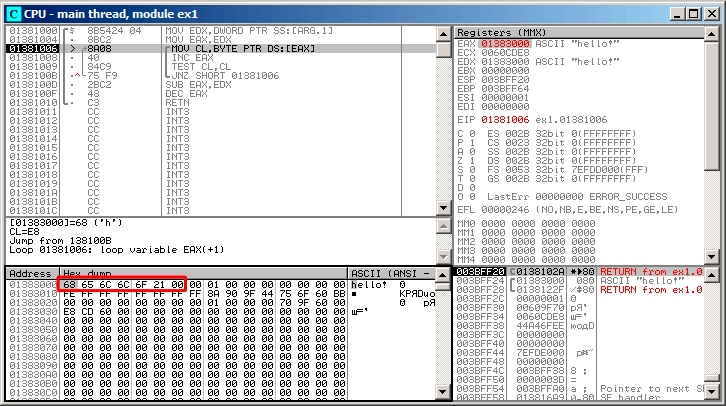
\includegraphics[scale=\FigScale]{patterns/10_strings/1_strlen/olly1.png}
\caption{\olly: \RU{начало первой итерации}\EN{first iteration start}}
\label{fig:strlen_olly_1}
\end{figure}

\RU{Видно, что \olly обнаружил цикл и, для удобства, \IT{свернула} инструкции тела цикла в скобке}
\EN{We see that \olly found a loop and, for convenience, \IT{wrapped} its instructions in brackets}.
\RU{Нажав правой кнопкой на}\EN{By clicking the right button on} \EAX, \RU{можно выбрать}\EN{we can choose} 
\q{Follow in Dump} 
\RU{и позиция в окне памяти будет как раз там, где надо.}
\EN{and the memory window scrolls to the right place.}
\RU{Здесь мы видим в памяти строку}\EN{Here we can see the string} \q{hello!}\EN{ in memory}.
\RU{После нее имеется как минимум 1 нулевой байт, затем случайный мусор}\EN{There is at least
one zero byte after it and then random garbage}.
\RU{Если \olly видит что в регистре содержится адрес какой-то строки, он показывает эту строку.}
\EN{If \olly sees a register with a valid address in it, that points to some string, 
it is shown as a string.}

\clearpage
\RU{Нажмем}\EN{Let's press} F8 (\stepover) \RU{столько раз, чтобы текущий адрес снова был 
в начале тела цикла}\EN{a few times, to get to the start of the body of the loop}:

\begin{figure}[H]
\centering
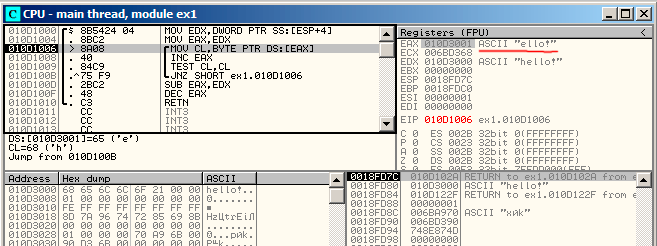
\includegraphics[scale=\FigScale]{patterns/10_strings/1_strlen/olly2.png}
\caption{\olly: \RU{начало второй итерации}\EN{second iteration start}}
\label{fig:strlen_olly_2}
\end{figure}

\RU{Видно, что}\EN{We see that} \EAX \RU{уже содержит адрес второго символа в строке}
\EN{contains the address of the second character in the string}.

\clearpage
\RU{Будем нажимать F8 достаточное количество раз, чтобы выйти из цикла:}
\EN{We have to press F8 enough number of times in order to escape from the loop:}

\begin{figure}[H]
\centering
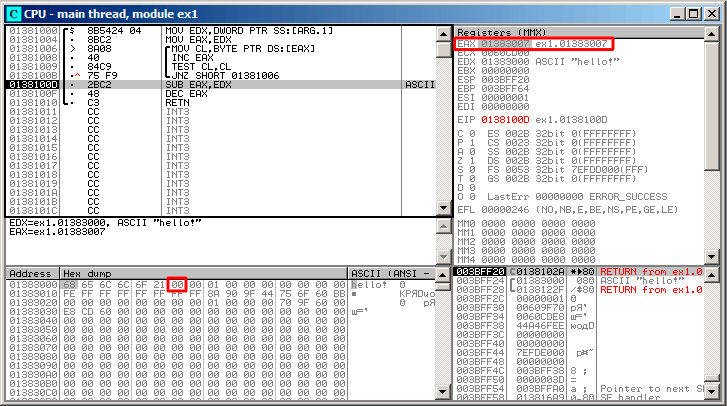
\includegraphics[scale=\FigScale]{patterns/10_strings/1_strlen/olly3.png}
\caption{\olly: \RU{сейчас будет вычисление разницы указателей}\EN{pointers difference to be calculated now}}
\label{fig:strlen_olly_3}
\end{figure}

\RU{Увидим, что \EAX теперь содержит адрес нулевого байта, следующего сразу за строкой}
\EN{We see that \EAX now contains the address of zero byte that's right after the string}.
\RU{А \EDX так и не менялся, он всё еще указывает на начало строки}\EN{Meanwhile, \EDX hasn't changed,
so it still pointing to the start of the string}.
\RU{Здесь сейчас будет вычисляться разница между этими двумя адресами.}
\EN{The difference between these two addresses is being calculated now.}

\clearpage
\RU{Инструкция \SUB исполнилась}\EN{The \SUB instruction just got executed}:

\begin{figure}[H]
\centering
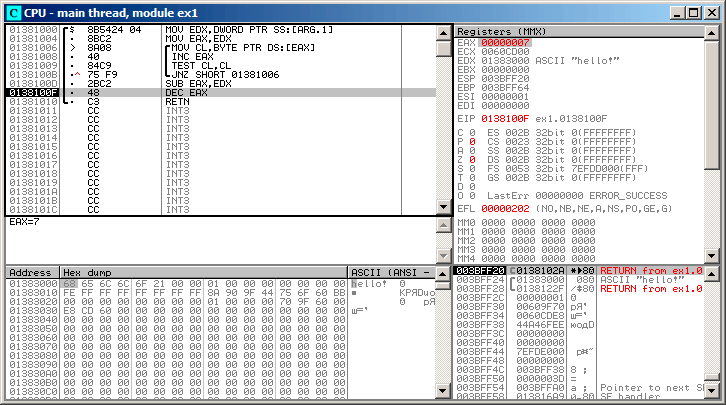
\includegraphics[scale=\FigScale]{patterns/10_strings/1_strlen/olly4.png}
\caption{\olly: \RU{сейчас будет декремент \EAX}\EN{\EAX to be decremented now}}
\label{fig:strlen_olly_4}
\end{figure}

\RU{Разница указателей сейчас в регистре \EAX --- 7.}
\EN{The difference of pointers is in the \EAX register now---7.}
\RU{Действительно, длина строки}\EN{Indeed, the length of the} \q{hello!} \RU{--- 6}\EN{string is 6}, 
\RU{но вместе с нулевым байтом}\EN{but with the zero byte included}\EMDASH{}7.
\RU{Но}\EN{But} \TT{strlen()} 
\RU{должна возвращать количество ненулевых символов в строке.}
\EN{must return the number of non-zero characters in the string.}
\RU{Так что сейчас будет исполняться декремент и выход из функции.}
\EN{So the decrement executes and then the function returns.}

\fi

\ifdefined\IncludeGCC
\subsubsection{\Optimizing GCC}

\RU{Попробуем GCC 4.4.1 с включенной оптимизацией (ключ \Othree):}
\EN{Let's check GCC 4.4.1 with optimizations turned on (\Othree key):}

\lstinputlisting{patterns/10_strings/1_strlen/10_3_gcc_O3.asm}

\RU{Здесь GCC не очень отстает от MSVC за исключением наличия \MOVZX.} 
\EN{Here GCC is almost the same as MSVC, except for the presence of \MOVZX.}

\RU{Впрочем, \MOVZX здесь явно можно заменить на}
\EN{However, here \MOVZX could be replaced with} \TT{mov dl, byte ptr [eax]}.

\RU{Но возможно, компилятору GCC просто проще помнить, что у него под переменную типа \Tchar отведен целый 
32-битный регистр \EDX и быть уверенным в том, что старшие биты регистра не будут замусорены.}
\EN{Probably it is simpler for GCC's code generator to \IT{remember} 
the whole 32-bit \EDX register 
is allocated for a \Tchar variable and it then can be sure that the highest bits has no any noise 
at any point.}

\label{strlen_NOT_ADD}
\index{x86!\Instructions!NOT}
\index{x86!\Instructions!XOR}
\RU{Далее мы видим новую для нас инструкцию \NOT. Эта инструкция инвертирует все биты в операнде. 
Можно сказать, что здесь это синонимично инструкции \TT{XOR ECX, 0ffffffffh}. 
\NOT и следующая за ней инструкция \ADD вычисляют разницу указателей и отнимают от результата единицу. 
Только происходит это слегка по-другому. Сначала \ECX, где хранится указатель на \IT{str}, 
инвертируется и от него отнимается единица.}
\EN{After that we also see a new instruction---\NOT. This instruction inverts all bits in the operand. 
You can say that it is a synonym to the \TT{XOR ECX, 0ffffffffh} instruction. 
\NOT and the following \ADD calculate the pointer difference and subtract 1, just in a different way. 
At the start \ECX, where the pointer to \IT{str} is stored, gets inverted and 1 is subtracted from it.}

\RU{См. также раздел:}\EN{See also:} \q{\SignedNumbersSectionName}~(\myref{sec:signednumbers}).

\RU{Иными словами, в конце функции, после цикла, происходит примерно следующее:} 
\EN{In other words, at the end of the function just after loop body, these operations are executed:}

\begin{lstlisting}
ecx=str;
eax=eos;
ecx=(-ecx)-1; 
eax=eax+ecx
return eax
\end{lstlisting}

\dots~\RU{что эквивалентно}\EN{and this is effectively equivalent to}:

\begin{lstlisting}
ecx=str;
eax=eos;
eax=eax-ecx;
eax=eax-1;
return eax
\end{lstlisting}

\RU{Но почему GCC решил, что так будет лучше? Снова не берусь сказать. Но я не сомневаюсь, 
что эти оба варианта работают примерно одинаково в плане эффективности и скорости.}
\EN{Why did GCC decide it would be better? I cannot be sure. 
But I'm sure the both variants are equivalent in efficiency.}
\fi
